

% =========================================================
\section{Algèbre de Boole}
% =========================================================

% --- Espace de Boole et variables ---
\begin{frame}{Espace de Boole et Variables Booléennes}

    \begin{block}{L'Espace de Boole \(\mathbb{B}\)}
        L'algèbre booléenne \footnote{L’algèbre de Boole est une algèbre au sens de structure algébrique, mais pas au sens d’algèbre sur un corps $\mathbb{K}$.} opère sur un ensemble à deux éléments :
        \[
            \mathbb{B} = \{0, 1\}
        \]
        où \(0\) représente \textbf{Faux} et \(1\) représente \textbf{Vrai}.
    \end{block}

    \vspace{0.4cm}

    \begin{columns}[T]
        \begin{column}{0.48\textwidth}
            \textbf{Variable booléenne simple}
            \begin{itemize}
                \item Une variable \(x\) qui ne peut prendre que deux valeurs.
                \item \(x \in \{0, 1\}\)
                \item Exemple : \textit{Un interrupteur est ouvert (0) ou fermé (1).}
            \end{itemize}
        \end{column}
        \begin{column}{0.48\textwidth}
            \textbf{Variable booléenne générale (vecteur)}
            \begin{itemize}
                \item Un vecteur de \(n\) bits : \(X = (x_{n-1}, \dots, x_0)\)
                \item \(X \in \mathbb{B}^n\)
                \item Exemple : \textit{Un octet (8 bits) représentant un état.}
            \end{itemize}
        \end{column}
    \end{columns}

\end{frame}

% --- Fonction booléenne ---
\begin{frame}{Fonction Booléenne}

    \begin{block}{Définition}
        Une \textbf{fonction booléenne} à \(n\) variables est une application :
        \[
            f : \mathbb{B}^n \to \mathbb{B}
        \]
        Elle associe à chaque combinaison d'entrées une unique sortie binaire.
    \end{block}

    \vspace{0.4cm}

    \begin{columns}[T]
        \begin{column}{0.55\textwidth}
            \textbf{Représentation}
            \begin{itemize}
                \item \textbf{Table de vérité} : énumère les \(2^n\) cas possibles.
                \item \textbf{Expression algébrique} : combinaison de \(+, \cdot, \bar{\phantom{x}}\).
            \end{itemize}

            \vspace{0.3cm}
            \textit{Exemple :} \(f(x,y) = x \cdot \bar{y} + \bar{x} \cdot y\) (XOR)
        \end{column}
        \begin{column}{0.4\textwidth}
            \centering
            \begin{tabular}{|c|c|c|}
                \hline
                \(x\) & \(y\) & \(f(x,y)\) \\
                \hline
                0 & 0 & 0 \\
                0 & 1 & 1 \\
                1 & 0 & 1 \\
                1 & 1 & 0 \\
                \hline
            \end{tabular}
        \end{column}
    \end{columns}

\end{frame}

% =========================================================
\section{Opérations}
% =========================================================

% --- Opérations fondamentales ---
\begin{frame}{Opérations Fondamentales}

    On utilise usuellement les symboles \(+\) pour le \textbf{OU} et \(\cdot\) (ou \(*\)) pour le \textbf{ET}.

    \vspace{0.3cm}

    \begin{columns}[T]
        \begin{column}{0.3\textwidth}
            \centering
            \textbf{Négation (NON)}\\
            \(\bar{x}\) ou \(\neg x\)
            \vspace{0.2cm}

            \begin{tabular}{|c|c|}
                \hline
                \(x\) & \(\bar{x}\) \\
                \hline
                0 & 1 \\
                1 & 0 \\
                \hline
            \end{tabular}
        \end{column}

        \begin{column}{0.35\textwidth}
            \centering
            \textbf{Conjonction (ET)}\\
            \(x \cdot y\) ou \(x * y\)
            \vspace{0.2cm}

            \begin{tabular}{|c|c|c|}
                \hline
                \(x\) & \(y\) & \(x \cdot y\) \\
                \hline
                0 & 0 & 0 \\
                0 & 1 & 0 \\
                1 & 0 & 0 \\
                1 & 1 & 1 \\
                \hline
            \end{tabular}
        \end{column}

        \begin{column}{0.35\textwidth}
            \centering
            \textbf{Disjonction (OU)}\\
            \(x + y\)
            \vspace{0.2cm}

            \begin{tabular}{|c|c|c|}
                \hline
                \(x\) & \(y\) & \(x + y\) \\
                \hline
                0 & 0 & 0 \\
                0 & 1 & 1 \\
                1 & 0 & 1 \\
                1 & 1 & 1 \\
                \hline
            \end{tabular}
        \end{column}
    \end{columns}

\end{frame}

% --- Opérateurs dérivés (aperçu) ---
\begin{frame}{Opérateurs Dérivés}

    Au-delà des trois opérations de base (\(+, \cdot, \bar{\phantom{x}}\)), on définit des \textbf{opérateurs dérivés} très utilisés en logique et en électronique.

    \vspace{0.4cm}

    \centering
    \begin{tabular}{|c|c|c|}
        \hline
        \textbf{Nom} & \textbf{Symbole} & \textbf{Expression en base} \\
        \hline
        OU exclusif (XOR) & \(x \oplus y\) & \(x \cdot \bar{y} + \bar{x} \cdot y\) \\
        NAND & \(x \uparrow y\) & \(\overline{x \cdot y}\) \\
        NOR & \(x \downarrow y\) & \(\overline{x + y}\) \\
        Équivalence (XNOR) & \(x \Leftrightarrow y\) & \(x \cdot y + \bar{x} \cdot \bar{y}\) \\
        Implication & \(x \Rightarrow y\) & \(\bar{x} + y\) \\
        \hline
    \end{tabular}

    \vspace{0.5cm}

    \begin{block}{Idée clé}
        Tous ces opérateurs se ramènent aux trois opérations fondamentales.
    \end{block}

\end{frame}

% --- XOR ---
\begin{frame}{Le OU Exclusif (\(x \oplus y\))}

    \begin{block}{Définition}
        « \(x\) ou \(y\), mais pas les deux » — noté \(x \oplus y\).
        \[
            x \oplus y \;=\; x \cdot \bar{y} + \bar{x} \cdot y
        \]
    \end{block}

    \vspace{0.4cm}

    \begin{columns}[T]
        \begin{column}{0.42\textwidth}
            \centering
            \begin{tabular}{|c|c|c|}
                \hline
                \(x\) & \(y\) & \(x \oplus y\) \\
                \hline
                0 & 0 & 0 \\
                0 & 1 & 1 \\
                1 & 0 & 1 \\
                1 & 1 & 0 \\
                \hline
            \end{tabular}
        \end{column}
        \begin{column}{0.55\textwidth}
            \textbf{Propriétés utiles :}
            \begin{itemize}
                \item \(x \oplus x = 0\)
                \item \(x \oplus \bar{x} = 1\)
                \item \(x \oplus 0 = x\)
                \item \(x \oplus 1 = \bar{x}\)
                \item \textbf{Associatif et commutatif}
            \end{itemize}

            \vspace{0.2cm}
            \textit{Application : addition binaire, détection de parité.}
        \end{column}
    \end{columns}

\end{frame}

% --- NAND et NOR ---
\begin{frame}{NAND et NOR : les Portes Universelles}

    \begin{columns}[T]
        \begin{column}{0.48\textwidth}
            \begin{block}{NAND (\(x \uparrow y\))}
                \[
                    x \uparrow y = \overline{x \cdot y}
                \]
                \centering
                \begin{tabular}{|c|c|c|}
                    \hline
                    \(x\) & \(y\) & \(x \uparrow y\) \\
                    \hline
                    0 & 0 & 1 \\
                    0 & 1 & 1 \\
                    1 & 0 & 1 \\
                    1 & 1 & 0 \\
                    \hline
                \end{tabular}
            \end{block}
        \end{column}

        \begin{column}{0.48\textwidth}
            \begin{block}{NOR (\(x \downarrow y\))}
                \[
                    x \downarrow y = \overline{x + y}
                \]
                \centering
                \begin{tabular}{|c|c|c|}
                    \hline
                    \(x\) & \(y\) & \(x \downarrow y\) \\
                    \hline
                    0 & 0 & 1 \\
                    0 & 1 & 0 \\
                    1 & 0 & 0 \\
                    1 & 1 & 0 \\
                    \hline
                \end{tabular}
            \end{block}
        \end{column}
    \end{columns}

    \vspace{0.4cm}

    \begin{alertblock}{Universalité}
        Toute fonction booléenne peut être réalisée en n'utilisant \textbf{que des NAND} ou \textbf{que des NOR}.
    \end{alertblock}

\end{frame}
% --- Équivalence ---
\begin{frame}{L'Équivalence (\(x \Leftrightarrow y\))}

    \begin{block}{Définition}
        « \(x\) si et seulement si \(y\) » — notée \(x \Leftrightarrow y\), également écrite \(x \leftrightarrow y\) ou XNOR.
        \[
            x \Leftrightarrow y \;=\; x \cdot y + \bar{x} \cdot \bar{y}
        \]
    \end{block}

    \vspace{0.4cm}

    \begin{columns}[T]
        \begin{column}{0.42\textwidth}
            \centering
            \begin{tabular}{|c|c|c|}
                \hline
                \(x\) & \(y\) & \(x \Leftrightarrow y\) \\
                \hline
                0 & 0 & 1 \\
                0 & 1 & 0 \\
                1 & 0 & 0 \\
                1 & 1 & 1 \\
                \hline
            \end{tabular}
        \end{column}
        \begin{column}{0.55\textwidth}
            \textbf{Points à retenir :}
            \begin{itemize}
                \item Vraie quand \(x\) et \(y\) sont \textbf{identiques}.
                \item C'est la \textbf{négation du XOR}.
                \item \(x \Leftrightarrow y = \overline{x \oplus y}\)
            \end{itemize}

            \vspace{0.3cm}
            \textit{Lien avec l'implication :}
            \[
                (x \Rightarrow y) \cdot (y \Rightarrow x) = x \Leftrightarrow y
            \]
        \end{column}
    \end{columns}

\end{frame}

% --- Implication : définition ---
\begin{frame}{L'Implication (\(x \Rightarrow y\)) : Définition}

    \begin{block}{Définition}
        « Si \(x\) alors \(y\) » — notée \(x \Rightarrow y\) ou \(x \to y\).
        \[
            x \Rightarrow y \;=\; \bar{x} + y
        \]
    \end{block}

    \vspace{0.4cm}

    \begin{columns}[T]
        \begin{column}{0.42\textwidth}
            \centering
            \begin{tabular}{|c|c|c|}
                \hline
                \(x\) & \(y\) & \(x \Rightarrow y\) \\
                \hline
                0 & 0 & 1 \\
                0 & 1 & 1 \\
                1 & 0 & \textbf{0} \\
                1 & 1 & 1 \\
                \hline
            \end{tabular}
        \end{column}
        \begin{column}{0.55\textwidth}
            \textbf{Un seul cas rend l'implication fausse :}
            \[
                x = 1 \quad \text{et} \quad y = 0
            \]

            \vspace{0.3cm}
            C'est le seul \textbf{contre-exemple} possible : l'antécédent est vrai mais la conclusion ne l'est pas.
        \end{column}
    \end{columns}

    \vspace{0.3cm}
    \centering
    \textit{Reformulation : \(x \Rightarrow y = \overline{x \cdot \bar{y}}\)\quad (négation d'un contre-exemple).}

\end{frame}

% --- Implication : paradoxe de l'antécédent faux ---
\begin{frame}{Implication : pourquoi est-elle vraie quand \(x = 0\) ?}

    \begin{alertblock}{La difficulté}
        Intuitivement, on se demande pourquoi \(0 \Rightarrow 0\) et \(0 \Rightarrow 1\) valent \(1\).
    \end{alertblock}

    \vspace{0.3cm}

    \textbf{Clé :} l'implication est une \textbf{contrainte conditionnelle}.

    \vspace{0.2cm}

    \[
        x \Rightarrow y \quad \text{signifie :} \quad \text{« \textbf{si} } x \text{ est vrai, \textbf{alors} } y \text{ doit être vrai. »}
    \]

    \vspace{0.3cm}

    \begin{itemize}
        \item Si \(x = 1\) : la contrainte s'applique. Il faut \(y = 1\), sinon elle est \textbf{violée}.
        \item Si \(x = 0\) : la contrainte \textbf{ne s'applique pas}. Elle n'est donc \textbf{pas violée}, donc elle est \textbf{vraie par défaut} (\textit{vacuité}).
    \end{itemize}

    \vspace{0.4cm}

    \begin{exampleblock}{Analogie météo}
        \textit{« S'il pleut, alors je prends mon parapluie. »}\\[0.2cm]
        Cette règle n'est \textbf{violée que dans un seul cas} : il pleut \textbf{et} je ne prends pas de parapluie.
    \end{exampleblock}

\end{frame}

% --- Implication : précaution d'usage + table météo ---
\begin{frame}[shrink=10] {Implication : Précaution d'Usage et Table Météo}

    \begin{alertblock}{Précaution d'usage}
        L'énoncé \textit{« S'il pleut, je prends mon parapluie »} doit être compris comme une \textbf{règle que je m'engage à suivre}, et non comme une \textbf{causalité physique}. De plus, il \textbf{ne dit rien} sur mon comportement quand il ne pleut pas.
    \end{alertblock}

    \vspace{0.1cm}

    \centering
    \renewcommand{\arraystretch}{1.3}
    \begin{tabular}{|c|c|c|l|}
        \hline
        \textbf{Il pleut} & \textbf{Parapluie} & \textbf{Règle} & \textbf{Interprétation} \\
        \(x\) & \(y\) & \(x \Rightarrow y\) & \\
        \hline
        1 & 1 & 1 & Règle respectée \\
        \textbf{1} & \textbf{0} & \textbf{0} & \textbf{Règle violée} \\
        0 & 1 & 1 & Pas de pluie — libre de mes choix \\
        0 & 0 & 1 & Pas de pluie — libre de mes choix \\
        \hline
    \end{tabular}

    \vspace{0.2cm}

    \begin{columns}[T]
        \begin{column}{0.48\textwidth}
            \textbf{Contraposition :}\\
            \(x \Rightarrow y \equiv \bar{y} \Rightarrow \bar{x}\)\\
            \textit{« Si je n'ai pas de parapluie,}\\
            \textit{alors il ne pleut pas. »}
        \end{column}
        \begin{column}{0.48\textwidth}
          \textbf{Identités remarquables :}
          \begin{align*}
            (0 \Rightarrow y) &= 1 \\
            (1 \Rightarrow y) &= y \\
            (x \Rightarrow 1) &= 1 \\
            (x \Rightarrow 0) &= \bar{x}
          \end{align*}
        \end{column}
    \end{columns}

\end{frame}

% --- Autres formes d'implication ---
\begin{frame}{Autres Formes d'Implication}

    \textbf{Règle de base :} \textit{« S'il pleut, je prends un parapluie. »} \quad (\(x \Rightarrow y\))

    \vspace{0.1cm}

    \begin{columns}[T]
        \begin{column}{0.45\textwidth}
            \begin{block}{Réciproque}
                \(y \Rightarrow x\)\\
                \textit{« Si je prends un parapluie, alors il pleut. »}\\
                \textbf{Non équivalente}.
            \end{block}

            \vspace{0.2cm}

            \begin{block}{Contraposée}
                \(\bar{y} \Rightarrow \bar{x}\)\\
                \textit{« Si je ne prends pas de parapluie, alors il ne pleut pas. »}\\
                \textbf{Équivalente} à la règle de base.
            \end{block}
        \end{column}
        \begin{column}{0.50\textwidth}
            \begin{block}{Réciproque de la contraposée}
                \(\bar{x} \Rightarrow \bar{y}\)\\
                \textit{« S'il ne pleut pas, je ne prends pas de parapluie. »}\\
                \textbf{Non équivalente}.
            \end{block}

            \vspace{0.2cm}

            \begin{block}{Équivalence}
                \((x \Rightarrow y) \cdot (y \Rightarrow x) = x \Leftrightarrow y\)\\
                \textit{« Je prends un parapluie si et seulement s'il pleut. »}
            \end{block}
        \end{column}
    \end{columns}

    \vspace{0.1cm}

    \begin{alertblock}{Piège classique}
        \centering
        \textbf{Confondre une implication avec sa réciproque est l'erreur logique la plus fréquente.}
    \end{alertblock}
\end{frame}


% --- Récapitulatif ---
\begin{frame}{Récapitulatif des Opérateurs Booléens}

    \centering
    \small
    \begin{tabular}{|c|c||c|c|c|c|c|c|}
        \hline
        \(x\) & \(y\) & \(\cdot\) & \(+\) & \(\oplus\) & \(\Leftrightarrow\) & \(\Rightarrow\) & \(\uparrow\) \\
        \hline
        0 & 0 & 0 & 0 & 0 & 1 & 1 & 1 \\
        0 & 1 & 0 & 1 & 1 & 0 & 1 & 1 \\
        1 & 0 & 0 & 1 & 1 & 0 & 0 & 1 \\
        1 & 1 & 1 & 1 & 0 & 1 & 1 & 0 \\
        \hline
    \end{tabular}

    \vspace{0.4cm}

    \begin{columns}[T]
        \begin{column}{0.48\textwidth}
            \textbf{Opérateurs de base :}
            \begin{itemize}
                \item ET (\(\cdot\)), OU (\(+\)), NON (\(\bar{\phantom{x}}\))
            \end{itemize}
        \end{column}
        \begin{column}{0.48\textwidth}
            \textbf{Opérateurs dérivés :}
            \begin{itemize}
                \item XOR, XNOR, implication, NAND, NOR
            \end{itemize}
        \end{column}
    \end{columns}

    \vspace{0.3cm}
    \centering
    \textit{16 fonctions booléennes à 2 variables existent  \footnote{Deux variables d'où 4 lignes et 2 choix pour \underline{chacune} des lignes : $2\times 2\times 2\times 2=2^4=16$}— celles-ci sont les plus utilisées.}

\end{frame}

% --- Priorité et parenthésage ---
\begin{frame}{Priorité des Opérations et Parenthésage}

    Comme en arithmétique, il existe un ordre de priorité implicite.

    \vspace{0.5cm}

    \begin{block}{Ordre de priorité (du plus fort au plus faible)}
        \begin{enumerate}
            \item \textbf{Négation} : \(\bar{x}\)
            \item \textbf{Conjonction} : \(x \cdot y\)
            \item \textbf{Disjonction} : \(x + y\)
        \end{enumerate}
    \end{block}

    \vspace{0.4cm}

    \textbf{Exemple :}
    \[
        \bar{x} \cdot y + z = \big((\bar{x}) \cdot y\big) + z
    \]

    \vspace{0.2cm}
    \centering
    \textit{En cas de doute, les parenthèses restent la meilleure amie du logicien.}

\end{frame}

% =========================================================
\section{Propriétés Algébriques}
% =========================================================

% --- Commutativité et associativité ---
\begin{frame}{Commutativité et Associativité}

    Les opérations \(+\) et \(\cdot\) possèdent des propriétés similaires à l'arithmétique classique.

    \vspace{0.4cm}

    \begin{block}{Commutativité}
        L'ordre des opérandes n'influence pas le résultat.
        \begin{align*}
            x + y &= y + x \\
            x \cdot y &= y \cdot x
        \end{align*}
    \end{block}

    \begin{block}{Associativité}
        L'ordre d'évaluation (groupement) n'influence pas le résultat.
        \begin{align*}
            (x + y) + z &= x + (y + z) \\
            (x \cdot y) \cdot z &= x \cdot (y \cdot z)
        \end{align*}
    \end{block}

\end{frame}

% --- Distributivité ---
\begin{frame}{Distributivité}

    \begin{alertblock}{Particularité de l'algèbre de Boole}
        Contrairement à l'arithmétique, le OU est distributif sur le ET \textbf{et réciproquement}.
    \end{alertblock}

    \vspace{0.4cm}

    \begin{columns}[T]
        \begin{column}{0.48\textwidth}
            \textbf{ET sur OU} (classique)
            \[
                x \cdot (y + z) = (x \cdot y) + (x \cdot z)
            \]
        \end{column}
        \begin{column}{0.48\textwidth}
            \textbf{OU sur ET} (surprenant !)
            \[
                x + (y \cdot z) = (x + y) \cdot (x + z)
            \]
        \end{column}
    \end{columns}

    \vspace{0.5cm}
    \centering
    \textit{Cette double distributivité est une signature de l'algèbre de Boole.}

\end{frame}

% =========================================================
\section{Théorèmes}
% =========================================================

% --- Théorèmes principaux ---
\begin{frame}{Théorèmes Principaux}

    Ces théorèmes permettent de simplifier les expressions logiques.

    \vspace{0.3cm}

    \begin{columns}[T]
        \begin{column}{0.48\textwidth}
            \textbf{Éléments Neutres}
            \begin{align*}
                x + 0 &= x \\
                x \cdot 1 &= x
            \end{align*}

            \vspace{0.2cm}

            \textbf{Éléments Absorbants}
            \begin{align*}
                x + 1 &= 1 \\
                x \cdot 0 &= 0
            \end{align*}
        \end{column}

        \begin{column}{0.48\textwidth}
            \textbf{Idempotence}
            \begin{align*}
                x + x &= x \\
                x \cdot x &= x
            \end{align*}

            \vspace{0.2cm}

            \textbf{Complémentation}
            \begin{align*}
                x + \bar{x} &= 1 \\
                x \cdot \bar{x} &= 0
            \end{align*}
        \end{column}
    \end{columns}

\end{frame}

% --- Absorption ---
\begin{frame}{Lois d'Absorption}

    \begin{block}{Définition}
        L'absorption permet d'éliminer des termes redondants dans une expression.
    \end{block}

    \vspace{0.5cm}

    \begin{columns}[T]
        \begin{column}{0.48\textwidth}
            \begin{align*}
                x + x \cdot y &= ? \\
                x \cdot (1 + y) &= x
            \end{align*}
        \end{column}
        \begin{column}{0.48\textwidth}
            \centering
            \textit{Intuition :}\\
            \vspace{0.2cm}
            Si \(x\) est vrai, l'expression est vraie\\
            quel que soit \(y\).
        \end{column}
    \end{columns}

    \vspace{0.5cm}

    \begin{exampleblock}{Exemple d'application}
        \[
            x + x \cdot y + x \cdot z = x \cdot (1 + y + z) = x
        \]
    \end{exampleblock}

\end{frame}

% --- Dualité ---
\begin{frame}{Principe de Dualité}

    \begin{alertblock}{Principe}
        Toute identité booléenne reste vraie si l'on échange simultanément :
        \[
            + \longleftrightarrow \cdot \qquad \text{et} \qquad 0 \longleftrightarrow 1
        \]
    \end{alertblock}

    \vspace{0.4cm}

    \textbf{Cela explique pourquoi les théorèmes vont souvent par paires :}

    \vspace{0.3cm}

    \centering
    \begin{tabular}{|c|c|}
        \hline
        \textbf{Identité} & \textbf{Identité duale} \\
        \hline
        \(x + 0 = x\) & \(x \cdot 1 = x\) \\
        \(x + 1 = 1\) & \(x \cdot 0 = 0\) \\
        \(x + x = x\) & \(x \cdot x = x\) \\
        \(\overline{x + y} = \bar{x} \cdot \bar{y}\) & \(\overline{x \cdot y} = \bar{x} + \bar{y}\) \\
        \hline
    \end{tabular}

\end{frame}

% --- De Morgan ---
\begin{frame}{Lois de De Morgan}

    Ces lois sont fondamentales pour la manipulation des expressions booléennes et la conception de circuits logiques.

    \vspace{0.4cm}

    \begin{alertblock}{Première Loi de De Morgan}
        La négation d'une disjonction est la conjonction des négations.
        \[
            \overline{x + y} = \bar{x} \cdot \bar{y}
        \]
    \end{alertblock}

    \vspace{0.2cm}

    \begin{alertblock}{Deuxième Loi de De Morgan}
        La négation d'une conjonction est la disjonction des négations.
        \[
            \overline{x \cdot y} = \bar{x} + \bar{y}
        \]
    \end{alertblock}

    \vspace{0.2cm}
    \centering
    \textit{En résumé : l'inverse d'une somme n'est pas la somme des inverses, mais le produit des inverses.}

\end{frame}
% =========================================================
\section{Application}
% =========================================================

% --- Exemple fil rouge : vote majoritaire ---
\begin{frame}{Exemple : Vote Majoritaire à 3 Personnes}

    \textbf{Énoncé :} Trois personnes votent. La décision est adoptée si \textbf{au moins deux} votent OUI.

    \vspace{0.4cm}

    \begin{columns}[T]
        \begin{column}{0.45\textwidth}
            \textbf{Variables :} \(a, b, c \in \{0,1\}\) (1 = OUI).

            \vspace{0.3cm}
            \textbf{Forme SOP (lignes où \(f=1\)) :}
            \[
                f = \bar{a}bc + a\bar{b}c + ab\bar{c} + abc
            \]
        \end{column}
        \begin{column}{0.5\textwidth}
            \centering
            \begin{tabular}{|c|c|c|c|}
                \hline
                \(a\) & \(b\) & \(c\) & \(f\) \\
                \hline
                0 & 0 & 0 & 0 \\
                0 & 0 & 1 & 0 \\
                0 & 1 & 0 & 0 \\
                0 & 1 & 1 & 1 \\
                1 & 0 & 0 & 0 \\
                1 & 0 & 1 & 1 \\
                1 & 1 & 0 & 1 \\
                1 & 1 & 1 & 1 \\
                \hline
            \end{tabular}
        \end{column}
    \end{columns}

\end{frame}

% --- Simplification de l'exemple ---
\begin{frame}{Simplification par les Théorèmes}

    \textbf{Expression initiale (SOP) :}
    \[
        f = \bar{a}bc + a\bar{b}c + ab\bar{c} + abc
    \]

    \vspace{0.3cm}

    \textbf{Étape 1 — Idempotence} (on duplique \(abc\)) :
    \[
        f = \bar{a}bc + a\bar{b}c + ab\bar{c} + abc + abc
    \]

    \vspace{0.2cm}

    \textbf{Étape 2 — Regroupement} :
    \[
        f = (\bar{a}bc + abc) + (a\bar{b}c + abc) + (ab\bar{c} + abc)
    \]

    \vspace{0.2cm}

    \textbf{Étape 3 — Distributivité} (\(x \cdot y + x \cdot \bar{y} = x\)) :
    \[
        f = bc + ac + ab
    \]

    \vspace{0.1cm}

    \begin{exampleblock}{Résultat : $f = ab + ac + bc$}
        % \[
        %     f = ab + ac + bc
        % \]
        Forme simplifiée bien plus économique à implémenter.
    \end{exampleblock}

\end{frame}

% --- Transition vers les circuits ---

% =========================================================
\section{Décomposition de Shannon et Formes Canoniques}
% =========================================================
% --- Frame : Décomposition de Shannon ---
\begin{frame}{Décomposition de Shannon}

    \begin{block}{Théorème — Expansion de Shannon }
        Toute fonction booléenne \(f : \mathbb{B}^n \to \mathbb{B}\) peut être décomposée par rapport à une variable \(x_i\) :
        \[
            f(\dots, x_i, \dots) = x_i \cdot f_{x_i=1} + \bar{x_i} \cdot f_{x_i=0}
        \]
        où \(f_{x_i=1}\) et \(f_{x_i=0}\) sont les \textbf{cofacteurs} de \(f\) par rapport à \(x_i\).
    \end{block}

    \vspace{0.1cm}

    \begin{columns}[T]
        \begin{column}{0.52\textwidth}
            \textbf{Forme duale (par rapport à \(+\)) :}
            \[
                f = (x_i + f_{x_i=0}) \cdot (\bar{x_i} + f_{x_i=1})
            \]

            \vspace{0.1cm}

            \textbf{Interprétation :}
            \begin{itemize}
                \item On \textbf{factorise} par \(x_i\).
                \item On évalue \(f\) dans les deux cas \(x_i = 1\) et \(x_i = 0\).
                \item Chaque cofacteur a une variable en moins.
                \item \texttt{BDD} en CAO : \textit{binary decision diagrams}.
            \end{itemize}
        \end{column}

        \begin{column}{0.45\textwidth}
            \begin{exampleblock}{Exemple : XOR}
                \(f(x,y) = x \oplus y \)

                \vspace{0.1cm}

                Décomposition par rapport à \(x\) :
                \begin{align*}
                    f_{x=1} &= \bar{y} \\
                    f_{x=0} &= y
                \end{align*}
                \[
                    f = x \cdot \bar{y} + \bar{x} \cdot y
                \]
            \end{exampleblock}
        \end{column}
    \end{columns}


\end{frame}

%\end{document}
% --- SOP / POS ---
\begin{frame}{Formes Canoniques : SOP et POS}

    \begin{columns}[T]
        \begin{column}{0.48\textwidth}
            \begin{block}{SOP (\textit{Sum of Products})}
                Somme de \textbf{mintermes} (produits où chaque variable apparaît une fois).
                \[
                    f = \bar{x} \cdot y + x \cdot \bar{y}
                \]
                Construite à partir des lignes où \(f = 1\).
            \end{block}
        \end{column}
        \begin{column}{0.48\textwidth}
            \begin{block}{POS (\textit{Product of Sums})}
                Produit de \textbf{maxtermes} (sommes où chaque variable apparaît une fois).
                \[
                    f = (x + y) \cdot (\bar{x} + \bar{y})
                \]
                Construite à partir des lignes où \(f = 0\).
            \end{block}
        \end{column}
    \end{columns}

    \vspace{0.5cm}

    \begin{exampleblock}{Lien avec la table de vérité}
        Toute fonction booléenne admet une unique forme canonique SOP et une unique forme canonique POS.
    \end{exampleblock}

\end{frame}

% =========================================================
\section{Tableau de Karnaugh}
% =========================================================
\begin{frame}{Tableau de Karnaugh : intuition}
  \begin{columns}
    \begin{column}{0.3\textwidth}
      \begin{itemize}
        \item \textbf{objectif} : simplifier une formule booléenne.
        \item \textbf{moyen} : disposition spatiale \textit{particulière}.
      \end{itemize}
    \end{column}
    \begin{column}{0.7\textwidth}
      \begin{center}
        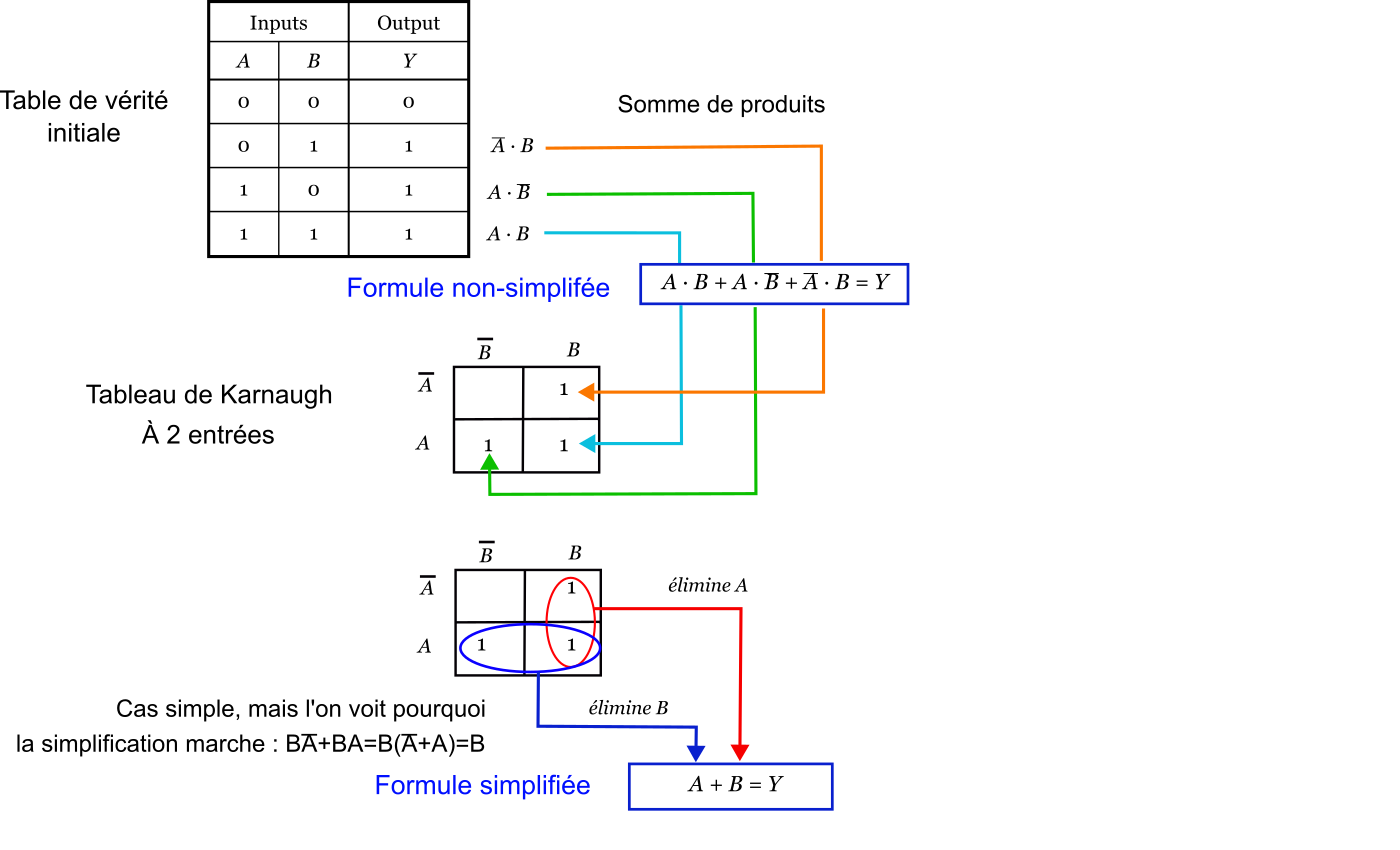
\includegraphics[scale=0.32]{./images/karnaugh_0.png}
      \end{center}
    \end{column}
  \end{columns}
\end{frame}

% --- Karnaugh : adjacence et principe ---
\begin{frame}{Tableau de Karnaugh : Adjacence et Principe}

    \begin{block}{Distance de Hamming}
        Pour deux vecteurs booléens \(u, v \in \mathbb{B}^n\), on définit :
        \[
            d_H(u,v) = \big|\{ i \in \{0,\dots,n-1\} : u_i \neq v_i \}\big|
        \]
        C'est le nombre de bits qui diffèrent entre \(u\) et \(v\).
    \end{block}

    \vspace{0.2cm}

    \begin{alertblock}{Définition — Adjacence}
        Deux cases du tableau de Karnaugh sont dites \textbf{adjacentes} si et seulement si : $d_H(u, v) = 1$
        % \[
        %     d_H(u, v) = 1
        % \]
        c'est-à-dire qu'elles ne diffèrent que par \textbf{une seule variable}.
    \end{alertblock}

    \vspace{0.1cm}

    \begin{columns}[T]
        \begin{column}{0.5\textwidth}
            \textbf{Justification :} si deux cases adjacentes ne diffèrent que par \(x\), leurs mintermes sont \(x \cdot m\) et \(\bar{x} \cdot m\), et :
            \[
                x \cdot m + \bar{x} \cdot m = (x + \bar{x}) \cdot m = m
            \]
            La variable \(x\) \textbf{disparaît}.
        \end{column}
        \begin{column}{0.45\textwidth}
            \textbf{Conséquence topologique :}\\
            Le tableau est \textbf{torique} — les bords opposés sont adjacents.

            \vspace{0.2cm}
            \textit{Exemple : \(000\) et \(100\) sont adjacents (\(d_H = 1\)).}
        \end{column}
    \end{columns}

\end{frame}

% --- Karnaugh : construction + code de Gray ---
\begin{frame}{Tableau de Karnaugh : Construction et Code de Gray}

    \begin{block}{Problème}
        Sur un tableau ordonné en binaire naturel, les cases voisines ne sont pas nécessairement adjacentes au sens de Hamming.
    \end{block}

    \vspace{0.3cm}

    \begin{columns}[T]
        \begin{column}{0.5\textwidth}
            \begin{alertblock}{Solution : Code de Gray}
                Ordonner les lignes et colonnes selon la suite :
                \[
                    00 \to 01 \to 11 \to 10
                \]
                Deux entrées consécutives diffèrent d'\textbf{un seul bit} (\(d_H = 1\)).
            \end{alertblock}
        \end{column}
        \begin{column}{0.45\textwidth}
            \centering
            \renewcommand{\arraystretch}{1.4}
            \begin{tabular}{|c|c|c|c|c|}
                \hline
                \(a \backslash bc\) & \(00\) & \(01\) & \textbf{\(11\)} & \(10\) \\
                \hline
                \(0\) & ~ & ~ & ~ & ~ \\
                \hline
                \(1\) & ~ & ~ & ~ & ~ \\
                \hline
            \end{tabular}
            % \begin{tabular}{|c|c|c|}
            %     \hline
            %     \(x \backslash y\) & \(0\) & \(1\) \\
            %     \hline
            %     \(0\) & \(\bar{x}\bar{y}\) & \(\bar{x}y\) \\
            %     \hline
            %     \(1\) & \(x\bar{y}\) & \(xy\) \\
            %     \hline
            % \end{tabular}

            \vspace{0.3cm}
            \textit{Chaque case = un minterme.}
        \end{column}
    \end{columns}

    \vspace{0.3cm}

    \textbf{Vérification :} \(00\) et \(01\) sont adjacents, \(01\) et \(11\) aussi, et ainsi de suite. La suite Gray garantit que toutes les cases voisines du tableau sont adjacentes au sens de Hamming.

\end{frame}

% --- Karnaugh : exemple 3 variables ---
\begin{frame}{Exemple : Tableau de Karnaugh à 3 Variables}

    \textbf{Fonction :} \(f(a,b,c) = \sum m(1,3,5,7)\)

    \vspace{0.3cm}

    \begin{columns}[T]
        \begin{column}{0.5\textwidth}
            \centering
            \renewcommand{\arraystretch}{1.6}
            \begin{tabular}{|c|c|c|c|c|}
                \hline
                \(a \backslash bc\) & \(00\) & \(01\) & \(11\) & \(10\) \\
                \hline
                \(0\) & 0 & \textbf{1} & \textbf{1} & 0 \\
                \hline
                \(1\) & 0 & \textbf{1} & \textbf{1} & 0 \\
                \hline
            \end{tabular}

            \vspace{0.3cm}

            \textit{Colonnes en code Gray : \(00, 01, 11, 10\).}
        \end{column}
        \begin{column}{0.48\textwidth}
            \textbf{Résolution :}

            \vspace{0.3cm}

            \begin{itemize}
                \item On regroupe les 4 \textbf{1} en un bloc \(2 \times 2\).
                \item Variables qui \textbf{changent} : \(a\) et \(b\).
                \item Variable qui \textbf{reste} : \(c = 1\).
                \item {\color{red} (Erreur dans le slideware distribué).} 
            \end{itemize}

            \vspace{0.4cm}

            \begin{exampleblock}{Résultat}
                \[
                    f = c
                \]
                De 4 mintermes à un seul littéral.
            \end{exampleblock}
        \end{column}
    \end{columns}


\end{frame}

% --- Karnaugh : regroupements formels ---
\begin{frame}{Regroupements : Règles Formelles}

    \begin{block}{Regroupement valide}
        Un regroupement est un sous-ensemble \(S\) de cases contenant des 1, tel que :
        \begin{itemize}
            \item \(|S| = 2^k\) pour un certain \(k \in \mathbb{N}\) ;
            \item \(S\) forme un \textbf{sous-cube} : produit cartésien de \(k\) paires d'entrées adjacentes.
        \end{itemize}
    \end{block}

    \vspace{0.3cm}

    \begin{alertblock}{Interprétation}
        Un sous-cube de taille \(2^k\) correspond à l'élimination de \(k\) variables par adjacence successive.
    \end{alertblock}

    \vspace{0.3cm}

    \begin{columns}[T]
        \begin{column}{0.5\textwidth}
            \textbf{Démarche :}
            \begin{enumerate}
                \item Remplir le tableau depuis la table de vérité.
                \item Identifier les \textbf{plus grands sous-cubes}.
                \item Vérifier que tous les 1 sont couverts.
                \item Lire le terme associé à chaque sous-cube.
            \end{enumerate}
        \end{column}
        \begin{column}{0.45\textwidth}
            \begin{exampleblock}{Limites}
                \begin{itemize}
                    \item Pratique jusqu'à 4 variables.
                    \item Difficile dès 5.
                    \item Au-delà : \textbf{Quine-McCluskey} ou \textbf{BDD}.
                \end{itemize}
            \end{exampleblock}
        \end{column}
    \end{columns}
\end{frame}
